\documentclass[logo,reportComp]{thesis}
\usepackage[cpp,pseudo]{mypackage}

\title{数字图像处理作业二}
\subtitle{}
\school{数据科学与计算机学院}
\author{陈鸿峥}
\classname{17大数据与人工智能}
\stunum{17341015}
\headercontext{数字图像处理作业}
\lstset{language=matlab}

\begin{document}

\maketitle
% PROJECT 03-02 03-05 03-06
本次作业包括拉普拉斯增强和锐化掩膜两个实验。
注意其中一些图片使用的是第三版的图片,所以实验结果可能存在差异。

\section{拉普拉斯增强(PROJECT 03-05)}
\subsection{原理}
利用
\[\nabla^2=\pd{f}{x}+\pd{f}{y}\]
的离散形式进行处理。
本例中采用如下掩膜进行计算。
\begin{center}
\begin{tabular}{|c|c|c|}\hline
-1 & -1 & -1\\\hline
-1 & 8 & -1 \\\hline
-1 & -1 & -1\\\hline
\end{tabular}
\end{center}

高斯滤波器模糊则是采用如下掩膜,其中$h(x,y)=\ee^{-\frac{x^2+y^2}{2\sigma^2}}$。
\begin{center}
\begin{tabular}{|c|c|c|}\hline
$h(-1,-1)$ & $h(-1,0)$ & $h(-1,1)$\\\hline
$h(0,-1)$ & $h(0,0)$ & $h(0,1)$ \\\hline
$h(1,-1)$ & $h(1,0)$ & $h(1,1)$\\\hline
\end{tabular}
\end{center}
注意实际实施时要先将掩膜归一化,避免最终的输出值超过255。

\subsection{实验结果与分析}
如图\ref{fig:a}所示,进行拉普拉斯锐化之后,图像边缘变得更加锋利,即实现了锐化的结果。
\begin{figure}[H]
\centering

\includegraphics[width=0.8\linewidth]{a.jpg}
\caption{(a)题结果}
\label{fig:a}
\end{figure}

如图\ref{fig:b}所示,经过不同方式进行图像锐化后结果都比原图像有了一定程度的提升。
\begin{figure}[H]
\centering

\includegraphics[width=\linewidth]{b.jpg}
\caption{(b)题结果}
\label{fig:b}
\end{figure}


\section{锐化掩膜(PROJECT 03-06)}
\subsection{原理}
反锐化掩膜得到的锐化图像是
\[f_s(x,y)=f(x,y)-\bar{f}(x,y)\]
高提升滤波得到的图像是
\[f_{hb}(x,y)=Af(x,y)-\bar{f}(x,y)\]

\subsection{实验结果与分析}
本题中$\bar{f}$采用均值滤波,$A$取$2$。
结果如图\ref{fig:res}所示,可以看到经过高提升滤波后,图像细节同样变得更加清晰。
\begin{figure}[H]
\centering
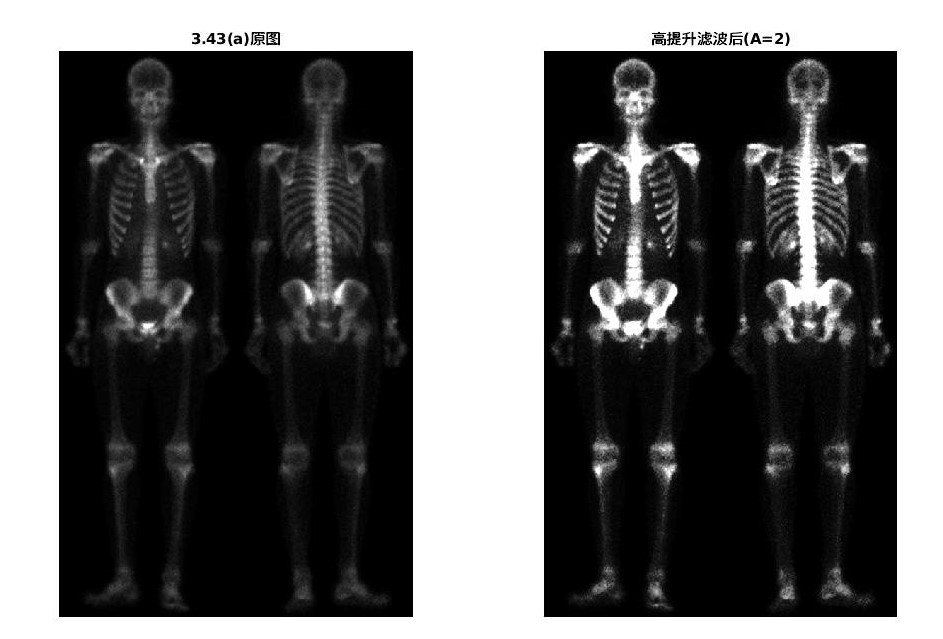
\includegraphics[width=\linewidth]{c.jpg}
\caption{高提升滤波结果}
\label{fig:res}
\end{figure}

\appendix\appendixconfig
\section{拉普拉斯增强}
\begin{lstlisting}
close all;clear all;clc;
I=imread('Fig0340.tif');
[m,n]=size(I);
newI=zeros(m,n);
for i = 2:m-1
    for j = 2:n-1
        newI(i,j)=-I(i+1,j)-I(i-1,j)-I(i,j+1)-I(i,j-1)+8*I(i,j)-I(i+1,j+1)-I(i+1,j-1)-I(i-1,j+1)-I(i-1,j-1);
    end
end
figure,
subplot(121),imshow(uint8(I));
title('`原图'')
subplot(122),imshow(uint8(newI));
title('`Laplacian变换后'');

sigma=3;
gauss=zeros(5,5);
sumup=0;
for i = -2:2
    for j = -2:2
        gauss(i+3,j+3)=exp(-(i*i+j*j)/(2*sigma*sigma));
        sumup = sumup + gauss(i+3,j+3); % normalization
    end
end
gauss=gauss./sumup;
newIb=zeros(m,n);
for i = 3:m-2
    for j = 3:n-2
        for u = -2:2
            for v = -2:2
                newIb(i,j) = newIb(i,j) + uint8(gauss(u+3,v+3)*I(i+u,j+v));
            end
        end
    end
end

newIc=zeros(m,n);
for i = 2:m-1
    for j = 2:n-1
        avg = 1/9*(I(i+1,j)+I(i-1,j)+I(i,j+1)+I(i,j-1)+I(i,j)+I(i+1,j+1)+I(i+1,j-1)+I(i-1,j+1)+I(i-1,j-1));
        newIc(i,j)=I(i,j)-uint8(avg);
    end
end

newId=zeros(m,n);
for i = 2:m-1
    for j = 2:n-1
        avg = 1/9*(I(i+1,j)+I(i-1,j)+I(i,j+1)+I(i,j-1)+I(i,j)+I(i+1,j+1)+I(i+1,j-1)+I(i-1,j+1)+I(i-1,j-1));
        newId(i,j)=2*I(i,j)-uint8(avg);
    end
end

newIe=zeros(m,n);
for i = 2:m-1
    for j = 2:n-1
        avg = 1/9*(I(i+1,j)+I(i-1,j)+I(i,j+1)+I(i,j-1)+I(i,j)+I(i+1,j+1)+I(i+1,j-1)+I(i-1,j+1)+I(i-1,j-1));
        newIe(i,j)=I(i,j)+4.5*(I(i,j)-uint8(avg));
    end
end

figure,
subplot(151),imshow(uint8(I));
title('`3.40(a)原图'')
subplot(152),imshow(uint8(newIb));
title('`高斯滤波'');
subplot(153),imshow(uint8(newIc));
title('`非锐化模板'');
subplot(154),imshow(uint8(newId));
title('`非锐化掩盖'');
subplot(155),imshow(uint8(newIe));
title('`高提升滤波'');
\end{lstlisting}

\section{锐化掩膜}
\begin{lstlisting}
close all;clear all;clc;
I=imread('Fig0343.tif');
[m,n]=size(I);
newI=zeros(m,n);
A=2;
for i = 2:m-1
    for j = 2:n-1
        avg = 1/9*(I(i+1,j)+I(i-1,j)+I(i,j+1)+I(i,j-1)+I(i,j)+I(i+1,j+1)+I(i+1,j-1)+I(i-1,j+1)+I(i-1,j-1));
        newI(i,j)=I(i,j)+A*(I(i,j)-uint8(avg));
    end
end
figure,
subplot(121),imshow(uint8(I));
title('`3.43(a)原图'')
subplot(122),imshow(uint8(newI));
title('`高提升滤波后(A=2)'');
\end{lstlisting}

\end{document}

% Suggested Format for Submitting Project Reports
% Because laboratory projects are in addition to course work, it is suggested that project
% reports be kept short, and be organized in a uniform manner to simplify grading. The
% following format achieves these objectives.

% Page 1. Cover Page. Typed or printed neatly.
% · Project title
% · Project number
% · Course number
% · Student's name
% · Date due
% · Date handed in
% · Abstract (not to exceed 1/2 page)

% Page 2. Technical discussion. One to two pages (max). This section should include the
% techniques used and the principal equations (if any) implemented.

% Page 3 (or 4). Discussion of results. One to two pages (max). A discussion of results
% should include major findings in terms of the project objectives, and make clear
% reference to any images generated.

% Results. Includes all the images generated in the project. Number images individually
% so they can be referenced in the preceding discussions.

% Appendix. Program listings. Includes listings of all programs written by the student.
% Standard routines and other material obtained from other sources should be
% acknowledged by name, but their listings should not be included.

% Layout. The entire report must be in standard sheet size format (8.5 x 11 inches in the
% U.S.) All sheets should be stapled in three locations to form a binding booklet-like
% support on the left margin. Alternatively, sheets can be assembled using a commercial
% plastic binding product with a clear plastic cover.

% A note on program implementation: As noted earlier, the objective of the computer
% programs used in the following projects is to teach the student how to manipulate
% images. There are numerous packages that perform some of the functions required to
% implement the projects. However, the use of "canned" routines as the only method to
% implement an entire project is discouraged. For example, if the students are using
% MATLAB and the Image Processing Toolbox, a balanced approach is to use MATLAB's
% programming environment to write M functions to implement the projects, using some of
% MATLAB's own functions in the process. A good example is the implementation of the 2-
% D Fourier Fast Transform. The student should use the MATLAB function that computes
% the 2-D FFT directly, but write functions for operations such as centering the transform,
% multiplying it by a filter function, and obtaining the spectrum.